% This is "sig-alternate.tex" V2.0 May 2012
% This file should be compiled with V2.5 of "sig-alternate.cls" May 2012
%
% This example file demonstrates the use of the 'sig-alternate.cls'
% V2.5 LaTeX2e document class file. It is for those submitting
% articles to ACM Conference Proceedings WHO DO NOT WISH TO
% STRICTLY ADHERE TO THE SIGS (PUBS-BOARD-ENDORSED) STYLE.
% The 'sig-alternate.cls' file will produce a similar-looking,
% albeit, 'tighter' paper resulting in, invariably, fewer pages.
%
% ----------------------------------------------------------------------------------------------------------------
% This .tex file (and associated .cls V2.5) produces:
%       1) The Permission Statement
%       2) The Conference (location) Info information
%       3) The Copyright Line with ACM data
%       4) NO page numbers
%
% as against the acm_proc_article-sp.cls file which
% DOES NOT produce 1) thru' 3) above.
%
% Using 'sig-alternate.cls' you have control, however, from within
% the source .tex file, over both the CopyrightYear
% (defaulted to 200X) and the ACM Copyright Data
% (defaulted to X-XXXXX-XX-X/XX/XX).
% e.g.
% \CopyrightYear{2007} will cause 2007 to appear in the copyright line.
% \crdata{0-12345-67-8/90/12} will cause 0-12345-67-8/90/12 to appear in the copyright line.
%
% ---------------------------------------------------------------------------------------------------------------
% This .tex source is an example which *does* use
% the .bib file (from which the .bbl file % is produced).
% REMEMBER HOWEVER: After having produced the .bbl file,
% and prior to final submission, you *NEED* to 'insert'
% your .bbl file into your source .tex file so as to provide
% ONE 'self-contained' source file.
%
% ================= IF YOU HAVE QUESTIONS =======================
% Questions regarding the SIGS styles, SIGS policies and
% procedures, Conferences etc. should be sent to
% Adrienne Griscti (griscti@acm.org)
%
% Technical questions _only_ to
% Gerald Murray (murray@hq.acm.org)
% ===============================================================
%
% For tracking purposes - this is V2.0 - May 2012

\documentclass{sig-alternate}

\usepackage{url}

\begin{document}
%
% --- Author Metadata here ---
\conferenceinfo{SOCM2013: Workshop on Theory and Practice of Social Machines, WWW2013}{2013, Rio de Janeiro, Brazil}
%\CopyrightYear{2007} % Allows default copyright year (20XX) to be over-ridden - IF NEED BE.
%\crdata{0-12345-67-8/90/01}  % Allows default copyright data (0-89791-88-6/97/05) to be over-ridden - IF NEED BE.
% --- End of Author Metadata ---

\title{Towards a classification framework for social machines}
%\subtitle{[Extended Abstract]
%\titlenote{A full version of this paper is available as
%\textit{Author's Guide to Preparing ACM SIG Proceedings Using
%\LaTeX$2_\epsilon$\ and BibTeX} at
%\texttt{www.acm.org/eaddress.htm}}}
%
% You need the command \numberofauthors to handle the 'placement
% and alignment' of the authors beneath the title.
%
% For aesthetic reasons, we recommend 'three authors at a time'
% i.e. three 'name/affiliation blocks' be placed beneath the title.
%
% NOTE: You are NOT restricted in how many 'rows' of
% "name/affiliations" may appear. We just ask that you restrict
% the number of 'columns' to three.
%
% Because of the available 'opening page real-estate'
% we ask you to refrain from putting more than six authors
% (two rows with three columns) beneath the article title.
% More than six makes the first-page appear very cluttered indeed.
%
% Use the \alignauthor commands to handle the names
% and affiliations for an 'aesthetic maximum' of six authors.
% Add names, affiliations, addresses for
% the seventh etc. author(s) as the argument for the
% \additionalauthors command.
% These 'additional authors' will be output/set for you
% without further effort on your part as the last section in
% the body of your article BEFORE References or any Appendices.

\numberofauthors{1} %  in this sample file, there are a *total*
% of EIGHT authors. SIX appear on the 'first-page' (for formatting
% reasons) and the remaining two appear in the \additionalauthors section.
%
\author{
% You can go ahead and credit any number of authors here,
% e.g. one 'row of three' or two rows (consisting of one row of three
% and a second row of one, two or three).
%
% The command \alignauthor (no curly braces needed) should
% precede each author name, affiliation/snail-mail address and
% e-mail address. Additionally, tag each line of
% affiliation/address with \affaddr, and tag the
% e-mail address with \email.
%
% 1st. author
\alignauthor
Authors\\
       \affaddr{Web and Internet Science Group}\\
       \affaddr{University of Southampton}\\
       \affaddr{Southampton, UK}\\
       \email{\{a,b,c,d,wh,nrs\}@ecs.soton.ac.uk}
}
% There's nothing stopping you putting the seventh, eighth, etc.
% author on the opening page (as the 'third row') but we ask,
% for aesthetic reasons that you place these 'additional authors'
% in the \additional authors block, viz.
%\additionalauthors{Additional authors: John Smith (The Th{\o}rv{\"a}ld Group,
%email: {\texttt{jsmith@affiliation.org}}) and Julius P.~Kumquat
%(The Kumquat Consortium, email: {\texttt{jpkumquat@consortium.net}}).}
%\date{30 July 1999}
% Just remember to make sure that the TOTAL number of authors
% is the number that will appear on the first page PLUS the
% number that will appear in the \additionalauthors section.

\maketitle
\begin{abstract}

The state of the art in human interaction with computation systems blurs the line between
computation performed by machine logic and algorithms, and those that result from input by
humans, arising from their own neurological processes and life experience. Current
socio-technical systems, known as `social machines' exploit the large-scale interaction of
humans with machines, motivated for numerous aims and purposes across the spectrums of
financial gain, charitable aid and simply for fun. In this paper we explore
the landscape of social machines, both past and present, towards the aim of defining an
initial classification framework. Through a number of knowledge elicitation
and refinement exercises we have identified the polyarchical relationship between
infrastructure, social machines and large-scale social initiatives. Our initial framework
describes classification constructs in the areas of {\it participation}, {\it participants} and
{\it motivation}. We present an initial classification of the largest social machines, as
an initial validation and demonstration of the use of our identified constructs.
There is rich potential for performing
analysis on the behaviour and phenomenology of social machines, and analysis of their
growth and outputs over time. Our future work is to elicit additional opinion,
classifications and validation from a wider audience, to produce a formal framework to
classify and aid in analysis of social machines.


\end{abstract}

% A category with the (minimum) three required fields
%\category{H.4}{Information Systems Applications}{Miscellaneous}
%A category including the fourth, optional field follows...
%\category{D.2.8}{Software Engineering}{Metrics}[complexity measures, performance measures]

%\terms{Theory}

%\keywords{ACM proceedings, \LaTeX, text tagging}

\section{Social machines: an introduction}
Once upon a time `machines' were programmed by programmers and used by users. The success of the Web has changed this relationship: we now see configurations of people interacting with content and with each other, typified by social Web sites. Rather than drawing a line through such Web-based systems to separate the human and digital parts (as computer science has traditionally done), we can now draw a line around them and treat each such compound as a `social machine' --- a machine in which the two aspects are seamlessly interwoven. This crucial transition in thinking acknowledges the reality of current socio-technical systems, and is essential to underpin any understanding of the science and engineering of their future development towards pervasive ecosystems of co-evolving social machines.

Essentially social machines can be characterised as assemblies of manually executed and machine-driven (as in `automatised') services and the interaction of such services. A traditional database, with users looking up records independently of each other and an administrator responsible for the management of the content, has some of the right ingredients, but there is really no social element in this strict provider-consumer relationship. When we fill out a form (e.g., health information, birds spotted in my garden, new construction sites on my way to work) the systems supporting this activity are minimal forms of social machines because the users are part of the `social computation', in this case the data creation and collection process facilitate through the site. This social component becomes richer when the database is curated by members of the broader community (e.g., Wikipedia) and when the social network adds value implicitly (e.g., Amazon) or explicitly (e.g., Facebook) to the overall system through their individual or joint activities.

A number of prominent examples aside, today we still see a divide between conventional IT systems dedicated to data- and computation-intensive tasks, and Web $2.0$ sites offering some combination of well-known participatory features, in which user-generated content and the underlying social network evolve dynamically and hand-in-hand. However, as technology becomes more and more ubiquitous, many of the challenges we witness in any domain of our life, business, and society will soon require solutions that rely on both of these axes: a sophisticated combination of data-intensive, complex automation and deep community involvement. This suggests the need for new types of systems to tackle these emerging challenges, and these systems will not be able to be built and used in a sustainable way without a through understanding of the science and engineering of (the continuum of) social machines.

As an early step towards achieving this principled understanding, we propose in this paper an initial outline for a classification framework for social machines. The primary aim of the framework is to identify and define the constructs to describe, study, and compare this expanding field of interdisciplinary research, as well as the increasing number of systems combining human and computational intelligence that are continuously being created in areas as diverse as traffic management, healthcare, media and journalism, or design and natural sciences.

The current version of our framework is the result of a knowledge elicitation process performed internally in our lab. Our goal is to present it to the broader community and extend and revise it based on their feedback in order to achieve a shared understanding of the basic notions and of the associated terminology, and to consensually lay out the structure of the design space that will enable a systematic study of existing and future social machines. We anticipate that the framework will be a useful tool for both researchers in social and computer sciences, and for developers and operators of social machines. Using a common conceptualisation allows the former to become familiar with the landscape, and identify topics of research that so far have remained unexplored or under-explored. They are given a theoretical grounding to observe the effects of specific technical properties of a system configuration on social behaviour, discover design and evolution patterns of such systems, learn about social network formation and dynamics, and devise incentive mechanisms to encourage wide participation. For developers and operators, the framework may inform the engineering of new systems in terms of critical features and community development.

This paper makes two main contributions: First, we introduce the notion of `social machines' and position it in connection to similar ideas and initiatives. Second we propose a set of constructs to capture the most important features of social machines and to compare existing instances thereof.

The remaining sections are organised as follows. In order to pin down what makes up a social machine, and establish the boundaries of this emerging field of research, we need to first understand the relationship between social machines and related topics such as human computation, collective intelligence, and crowdsourcing; Section \ref{sec:comparison} gives a summary of this comparative analysis. In Section \ref{sec:framework} we then present the framework in terms of the methodology used to devise it, the main clusters of constructs used for classification, and an example of using them to compare a selection of popular social machines via grid analysis. We conclude with an outlook of our future development activities, including details about the evaluation of the framework. In addition, we plan to engage with the broader community to set up a `social machine' bringing together researchers from various disciplines who will contribute to the `computation' of a joint and widely agreed classification framework for the field.

\section{Comparison with related fields}
\label{sec:comparison}
Since the invention of the Turing machine we have experienced a `paradigm shift' in the usage of computers, moving away from purely calculative devices to facilitators of a wide range of human interactions. The emergence of `Computer-supported Collaboration Work (CSCW)' \cite{grudin1994computer} is representative for the early days of this trend. CSCW addresses `how collaborative activities and their coordination can be supported by means of computer systems' \cite{grudin1994computer}, whereas the initial concept evolved towards the more broader field of `Computer-supported collaboration' (CSC).

The Web as a global platform for information access and sharing marked a second essential milestone; in particular, through principles and technologies promoted through Web $2.0$ and the Mobile Web. These developments led to amazing growth in terms of the amounts of content available online and mass participation. They are responsible for hundreds of millions of users all over the globe creating high-quality encyclopaedias, publishing Terabytes of multimedia content, contributing to world-class software, and lively taking part in defining the agenda of many aspects of our society. This trend towards `prosumerism' is finding more and more adopters in the public and private sector as well, as governments and enterprises not only become active in open initiatives, but encourage the participation of their customers and employees in taking decisions related to organisational management, product development, services offers, and policies. In this context, a number of terms are used to refer to the ways people interact with each other and with applications: `wisdom of the crowds', `collective intelligence', `open innovation', `crowdsourcing', `human computation', and `social computing'. They are related, but not synonymous with `social machines', as explained in the following (see also Figure \ref{fig:socialmachine}).

\begin{figure}[htb]
\begin{center}
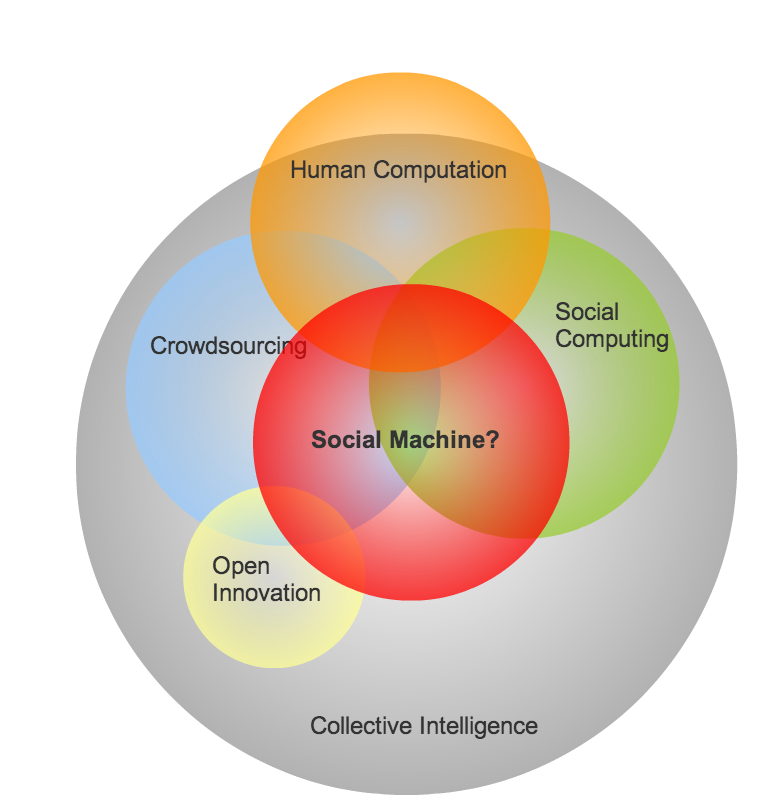
\includegraphics[width=0.25\textwidth]{img/socialmachinescope.png}
\caption{Social machines and related areas} \label{fig:socialmachine}
\end{center}
\end{figure}

Wisdom of the crowds \cite{surowiecki2005wisdom} refers to a principle for decision making that takes into account information and opinions of a group of people rather than individuals; the use of specific technologies, most notably Web $2.0$, has made it possible for such processes to be carried out at scales hardly conceivable in the past, and to involve highly diverse and geographically distributed participants. A similar concept, though broader scoped, is collective intelligence, defined in \cite{malone2009harnessing} as `groups of individuals doing things collectively that seem intelligent.' The main difference to what we refer to as `social machines' is hidden in the the automation part of the latter. In a social machine, human and computational intelligence coalesce in order to achieve a given purpose. The overall setting may slightly vary in terms of the interaction patterns between the two types of services and the way their outcomes are used; however, where wisdom of the crowds and collective intelligence clearly place their focus on identifying the situations in which groups of people perform better than individuals, social machines are concerned with the study and realisation of hybrid systems where the two types of components co-exist. As such, theoretical and empirical insights from the two related areas are useful to understand the dynamics of the social structures underlying such a system, but they are definitely not the only ingredient needed to build operational social machines. The question of how human and automatic services can be brought together to achieve optimal results, as well as the actual engineering exercise by which a system is developed, tested, and updated are equally important.

One of the direct consequences of the popularity of the wisdom of the crowds idea was a stronger investment worldwide in open innovation, which can be seen as an application of the concept to business environments, or, in the words of the authors, as a `a paradigm that assumes that firms can and should use external ideas as well as internal ideas, and internal and external paths to market, as the firms look to advance their technology' \cite{chesbrough2003}. At a more general level, this kind of creativity could be leveraged in almost any domain which benefits from diversity, while in the same time ensuring in-time access of a potentially infinite pool of skills and resources not available before the advent of social computing technologies. The term crowdsourcing is typically associated with this larger collection of situations, in which `a job traditionally performed by a designated agent [...] [is outsourced] to an undefined, generally large group of people in the form of an open call' \cite{howe2006crowdsourcing}. Human computation applies human processing power to tackle technical tasks that computers (still) find challenging \cite{von2009human}, typically in areas such as visual, audio, and natural language understanding. This sort of tasks are an important part of today's crowdsourcing projects landscape, in particular on so-called `microtask' platforms such as Amazon's Mechanical Turk\footnote{\url{https://www.mturk.com/}} or CrowdFlower\footnote{\url{http://crowdflower.com/}}, which offer small financial rewards to an anonymous crowd engaged with atomic units of work in the range of seconds to minutes to complete. The key difference between social machines and open innovation and crowdsourcing is again in the computational part. The novelty these two approaches bring in lies in using a much larger pool of human resources as traditional work environments \cite{quinn2011human}. There are clear socio-economic implications that their adopters need to deal with in order to optimally make use of this wealth of resources; technology may be needed to assist specific aspects of crowdsourcing projects, from evaluating and rewarding the results produced by the crowd to consolidating and aggregating them into a complete solution. A principled combination of human and computational capabilities is less in the focus of such systems and the technical means that support them, by contrast to social machines. In comparison to human computation, social machines cover a wider range of scenarios. Human computation is AI-centric and uses people to perform tasks that computers are not (yet) able to tackle (in terms of accuracy) \cite{quinn2011human}; by comparison, we see many successful examples of social machines in which the role of machines is rather to facilitate interactions within groups of people or communities of interest.

An analogous line of reasoning could be followed to point out the overlaps between social machines and social computing \cite{parameswaran2007research}. The latter is an area of computer science which refers systems that support `the gathering, representation, processing, use, and dissemination of information that is distributed across social collectivities such as teams, communities, organisations, and markets' \cite{parameswaran2007research}. As such, compared to the general concept of `Computer-supported collaboration', social computing puts a greater emphasis on the information management capabilities of groups and communities, and less on the way these capabilities emerge as a joint effort. This distinction is even stronger in the case of social machines, which look at the social and the technical components as equal and necessary partners, and study the ways they could be best combined to master the challenges of future socio-technical systems.

We now turn to a description of the main classification dimensions and features relevant to describe, study, and compare social machines.

\section{Classification of social machines}
\label{sec:framework}

\subsection{Methodology}
\label{sec:methodology}
The classification framework presented in this paper was created through knowledge elicitation ~\cite{knowledgeelicitation}. In particular we used the {\it repertory grid} elicitation
technique~\cite{kelly} in order to derive an initial set of {\it elements}, which represent instances of social machines, and {\it constructs}, which capture their most important characteristics.
In repertory grid elicitation a software tool is used to ask users to describe constructs
that differentiate between elements -- for example, prompting the user to create a construct that
differentiates between {\it GalaxyZoo}\footnote{In GalaxyZoo people classify galaxies with collective performance as good as professional astronomers, see \url{http://www.galaxyzoo.org}.} and {\it Facebook}, as two prominent example of social machines our classification framework should apply to. The user describes the opposing poles of the construct -- in this case, the user may decide on `For Science' and `For socialising' in order to capture the core distinction between the two system. The user then rates every element with value from $1$ to $5$ on this construct, where $1$ represents an element that is purely
`For Science', and $5$ one that mainly serves `socialising' purposes. Elements can also be rated with values between the poles if they may correspond to both or neither. The repertory grid software then identifies elements that are the least differentiated when requesting new constructs, in an attempt to elicit as much knowledge as possible from the user. We applied this technique to create an initial set of examples of social machines and to classify them according to specific features. To do so, we asked then computer science researchers familiar with the field to create their own repertory grids, and populate the elements from their own knowledge, and created the constructs using the standard repertory grid elicitation technique described above. This exercise led to $10$ grids, the union of which comprised a total of $56$ unique elements (social machines)
and $117$ different constructs (classifying factors). As the aim of this initial phase was to understand how people perceive the notion of social machine and their most distinctive properties, we allowed the participants to choose the social machines they are familiar with and describe them in their own terms.

%To enrich the resulting list of classifying constructs we then extracted the most frequent tags used in connection to the $56$ systems mentioned by the participants from the online bookmarking service {\it delicious.com}, thus achieving a crowdsourced social-machine classification containing the following clusters: Social Networks, (Micro)Blogging, News Aggregators, Image Boards, Crowd Science, Answer Gardens, Community Watch, Health and Wellbeing Support, Action and Investigation, Opinion Sharing, Video Sharing, Photo Sharing, Code Sharing, Art Sharing, Crowdsourcing Platforms, Mash-up Systems, and Crowdsourcing Toolkits and Platforms.

While determining the intersection of elements was straightforward, the consolidation of the
constructs required a more thorough process. We manually grouped the constructs into rough clusters, based around the areas they cover. We examined each construct to determine which were equivalent, and whether we could re-word or subsume existing constructs to cover the same aspects. The aim of this exercise was twofold: to remove any redundancy and cut the classification space down to a manageable size, while ensuring that all constructs that were elicited were represented in the final set. This process involved four of the authors discussing the choices, and resulted in a consolidated set of $31$ constructs organised in four different clusters: popularity, tasks and purpose, participants and roles, and motivation and incentives. In our analysis we will not further consider the first cluster, which primarily covered descriptive information about a given system, such as its perceived level of maturity and current number of users. Further on, the constructs were not evenly distributed across clusters; whereas some aspects such as roles of participants occurred frequently (in various flavours) in the grids provided by the ten experts, others such as the different types of workflows synthesising human and automatised capabilities of a social machine were less taken into account. As discussed in Section \ref{sec:comparison} we believe that the interaction between these two types of services is an essential part of the theory and practice of social machines, being one of the elements that distinguishes them from related areas which are biased towards one or the other. Extending the framework with constructs capturing these aspects (see, for instance, \cite{quinn2011human} for examples in the context of human computation) is part of our future work.

The paper presents the current version of the framework. We envision a reiteration of the main clusters and constructs based on discussions with and feedback from various scientific audiences. We provide initial evidence of the usability of the framework as a tool to examine commonalities and differences between social machines in Section \ref{sec:usage}, in which we applied the repertory grid elicitation technique to a set of $20$ social machines instances ranked by popularity according to the Alexa service.\footnote{\url{www.alexa.com/}} A more thorough evaluation will determine the extent to which the classification constructs identified can be meaningfully used by researchers and system designers and operators. We will test the completeness, correctness, and comprehensibility of the constructs in experiments in which a new set of social machines will be classified by framework users; we will ask the participants to assess the quality of the framework along these general dimensions, and measure inter-annotator agreement to learn about the usefulness of the classifications produced.

\subsection{The polyarchical relationship of social machines}
When defining the boundaries of what we call social machines, one important observation was related to the distinction between platforms and technologies such as wikis and GWAP (`games-with-a-purpose'), which enable social machines to be created, and their instantiations into social machines that were brought to life for a specific purpose, such as Wikipedia and EteRNA\footnote{\url{http://eterna.cmu.edu}}, a game in which participants design RNA that is evaluated automatically using simulators. A second observation is concerned with the relationship between broader and narrower-scoped instances of social machines; general-purpose examples such as Facebook, Twitter or Amazon, or even the Web, enable the formation of more specific social machines and communities within them, that are working to solve solve different problems. An example illustrating this relationship is the Obama'12 US Presidential campaign~\cite{obamakieron}, which relied on Twitter and Facebook as basic social machines; most forms of customer relationship management and community engagement carried out in the digital space use similar tools. Finally, social machines are interconnected into a greater ecosystem, both at the social and at the computation levels. For example, insights on the classification of space objects gained through GalaxyZoo may influence the content of the corresponding articles, and the associated editorial processes, within Wikipedia. In the same time,a large number of communities within Wikipedia focus specific topics and activities, such as those contributing to science and technology.\footnote{Visualisation of Wikipedia Science Communities: \url{http://www.olihb.com/WikiCommunities/}}

Looking at the set of social machines in a polyarchy leads to a broad/specific relationship emerging that lets us talk about behaviour at various levels of granularity. We propose looking at nested machines with `The Web' as one of several potential roots, with the next level down consisting of sub-platforms (such as Facebook, Twitter, MediaWiki, Ushahidi) that spawn more specific social machines. A resulting polyarchy is shown in Figure~\ref{polyarchy}, which classifies levels as infrastructure, frameworks, services, and projects and initiatives.

\begin{figure}[htb]
\begin{center}
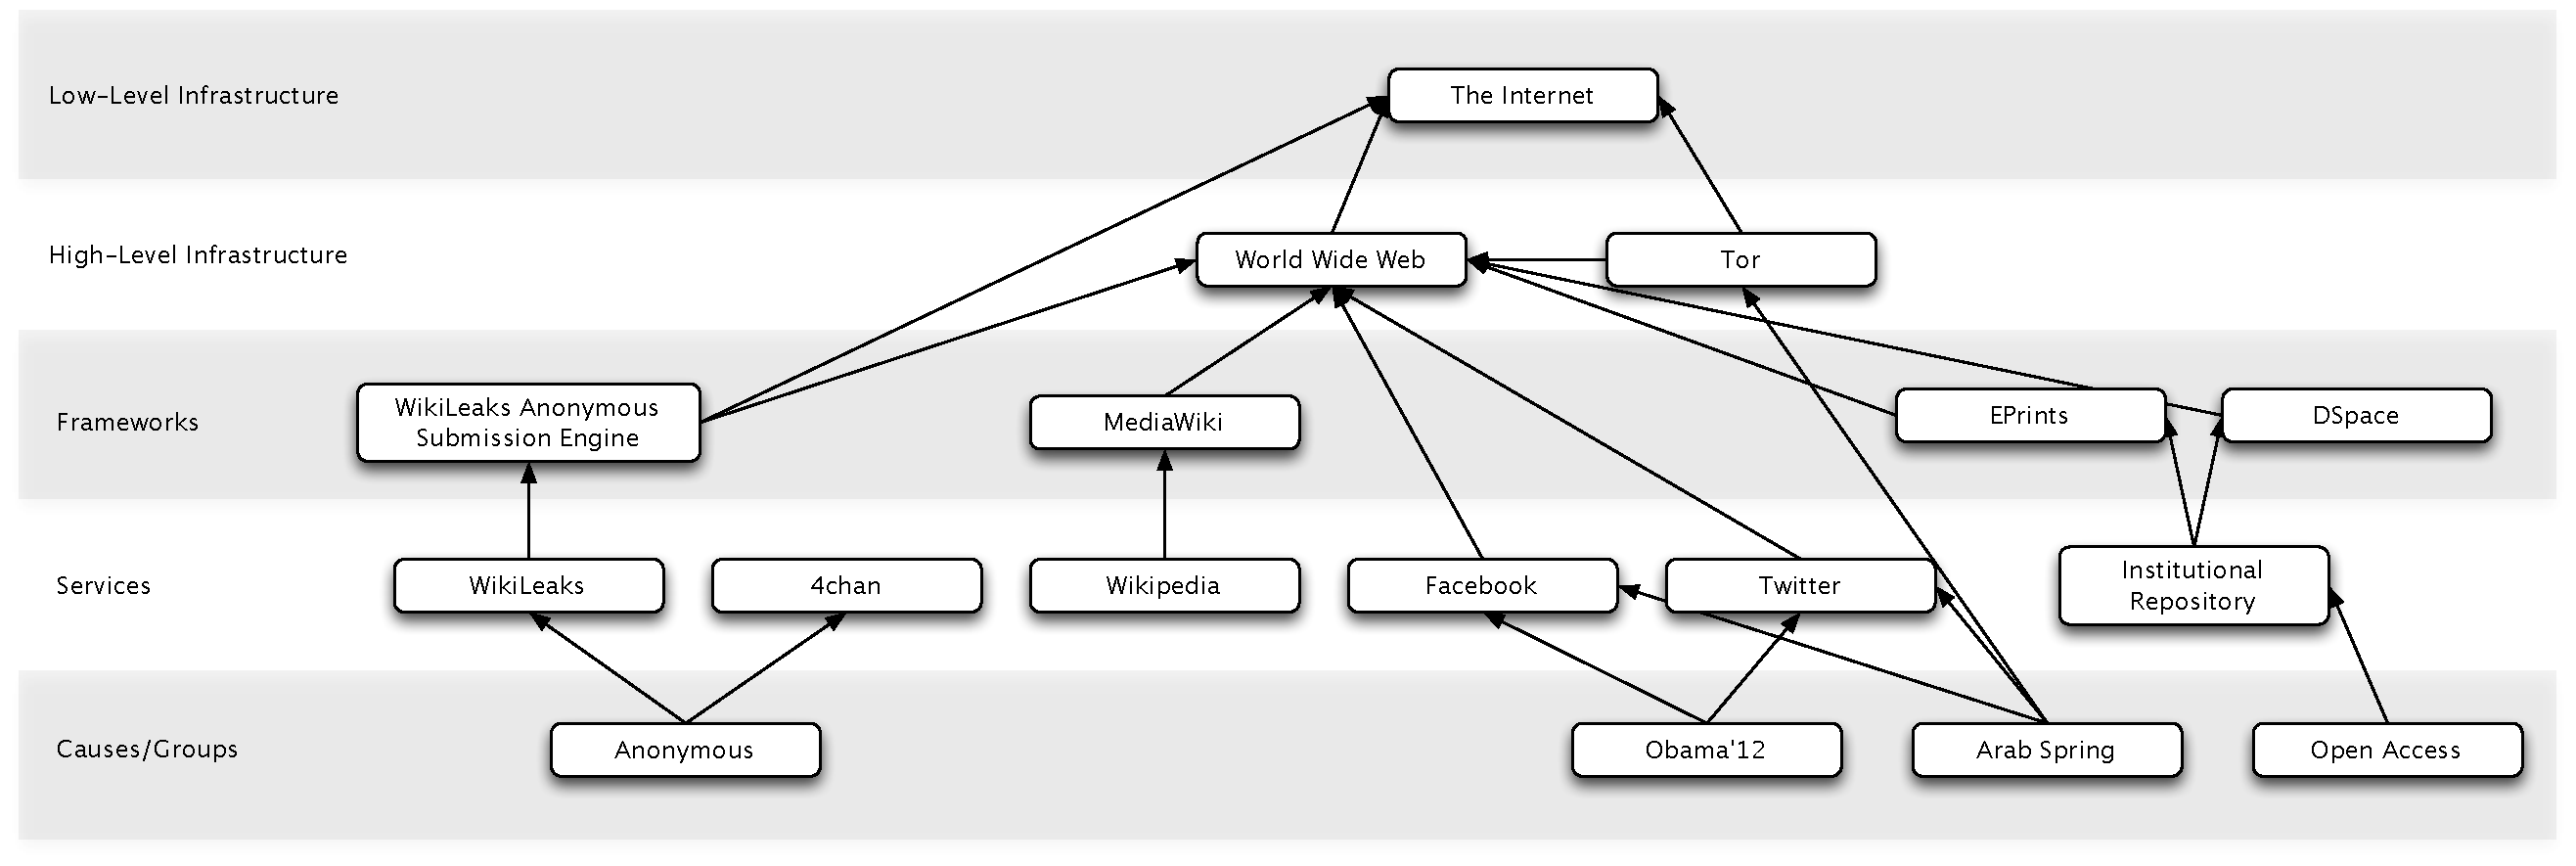
\includegraphics[width=0.4\textwidth]{img/polyarchy.pdf}
\caption{A polyarchy of social machines, illustrating the infrastructure and frameworks used by social machines, and machine-machine usage} \label{polyarchy}
\end{center}
\end{figure}

This approach enables us to start with a more detailed analysis of certain levels over others;
and seeing what similarities flow up and down the polyarchy. For example, what do
specific instances of Ushahidi/Zooniverse/MediaWiki have in common with other instances, and
how to they differ dynamically? How do certain design decisions taken at the level of the infrastructure, frameworks and service propagate into narrower-focused systems that are built on top of them? Similarly, how will such decisions affect a broader ecosystem of social machines, each with their own, though overlapping, purposes and communities?

The polyarchy is complementary to the classification constructs we elicited. The constructs apply to all levels of the polyarchy, though some of them might be more easier to understand and describe in the context of some levels. For example, instances of social machines residing at the bottom of the polyarchy are likely to be built with a very concrete audience in mind, and as such the mechanisms to incentivise participation are likely to be clearer and more straightforward to study and adjust than in cases in which such boundaries cannot be defined, such as Facebook, or even Wikipedia. In the same time, these systems will have to decide among an array of diverse basic services and frameworks for their implementations; the impact of such engineering decisions is difficult to predict in great detail as a thorough understanding of what makes certain social machines more successful than others, in terms of technology choices and beyond, is largely missing for most application domains.

%One such example is the `open access' movement in scholarly publishing
%~\cite{harnad2001self}. This cause mobilises academic authors to self-archive their own papers online so they are available for free, in addition to hosted versions behind publishers pay-walls. In order to achieve this aim, the social machine of `open access' typically uses the social machines of institutional repositories provided
%by the authors' associated institutions. As with other social machines, these social
%machines typically use off-the-shelf implementations (in this case the most popular are
%EPrints~\cite{eprints} and DSpace~\cite{dspace}), which run as web sites on the world wide
%web. This cause is mature, growing year-on-year and has global coverage.


%One originally unforeseen classification is that of the causes that utilise Social Machines.
%Through a particularly popular cause, large numbers of participants can be mobilised, for
%either a short period of time, or for long-term engagement, using multiple social machines
%in order to further their cause. Examples of causes can be seen in Figure~\ref{polyarchy},
%at the lowest level of the polyarchy.
%\subsubsection{Multi-faceted motivation, and who-gets-what benefit}
%
%%We identified a hierarchy of constructs pertaining to the motivation people have for using social
%%machines with top level constructs of:
%%
%%\begin{enumerate}
%%\item Hedonistic
%%\item Financial
%%\item To be informed
%%\item To help others
%%\end{enumerate}
%%
%%The sub constructs are illustrated in Figure~\ref{motivation}, and we relate them to Maslow's hierarchy of needs~\cite{maslow}, (e.g., self-actualisation, security, respect of others), in various ways.
%%
%%\begin{figure*}[htb]
%%\begin{center}
%%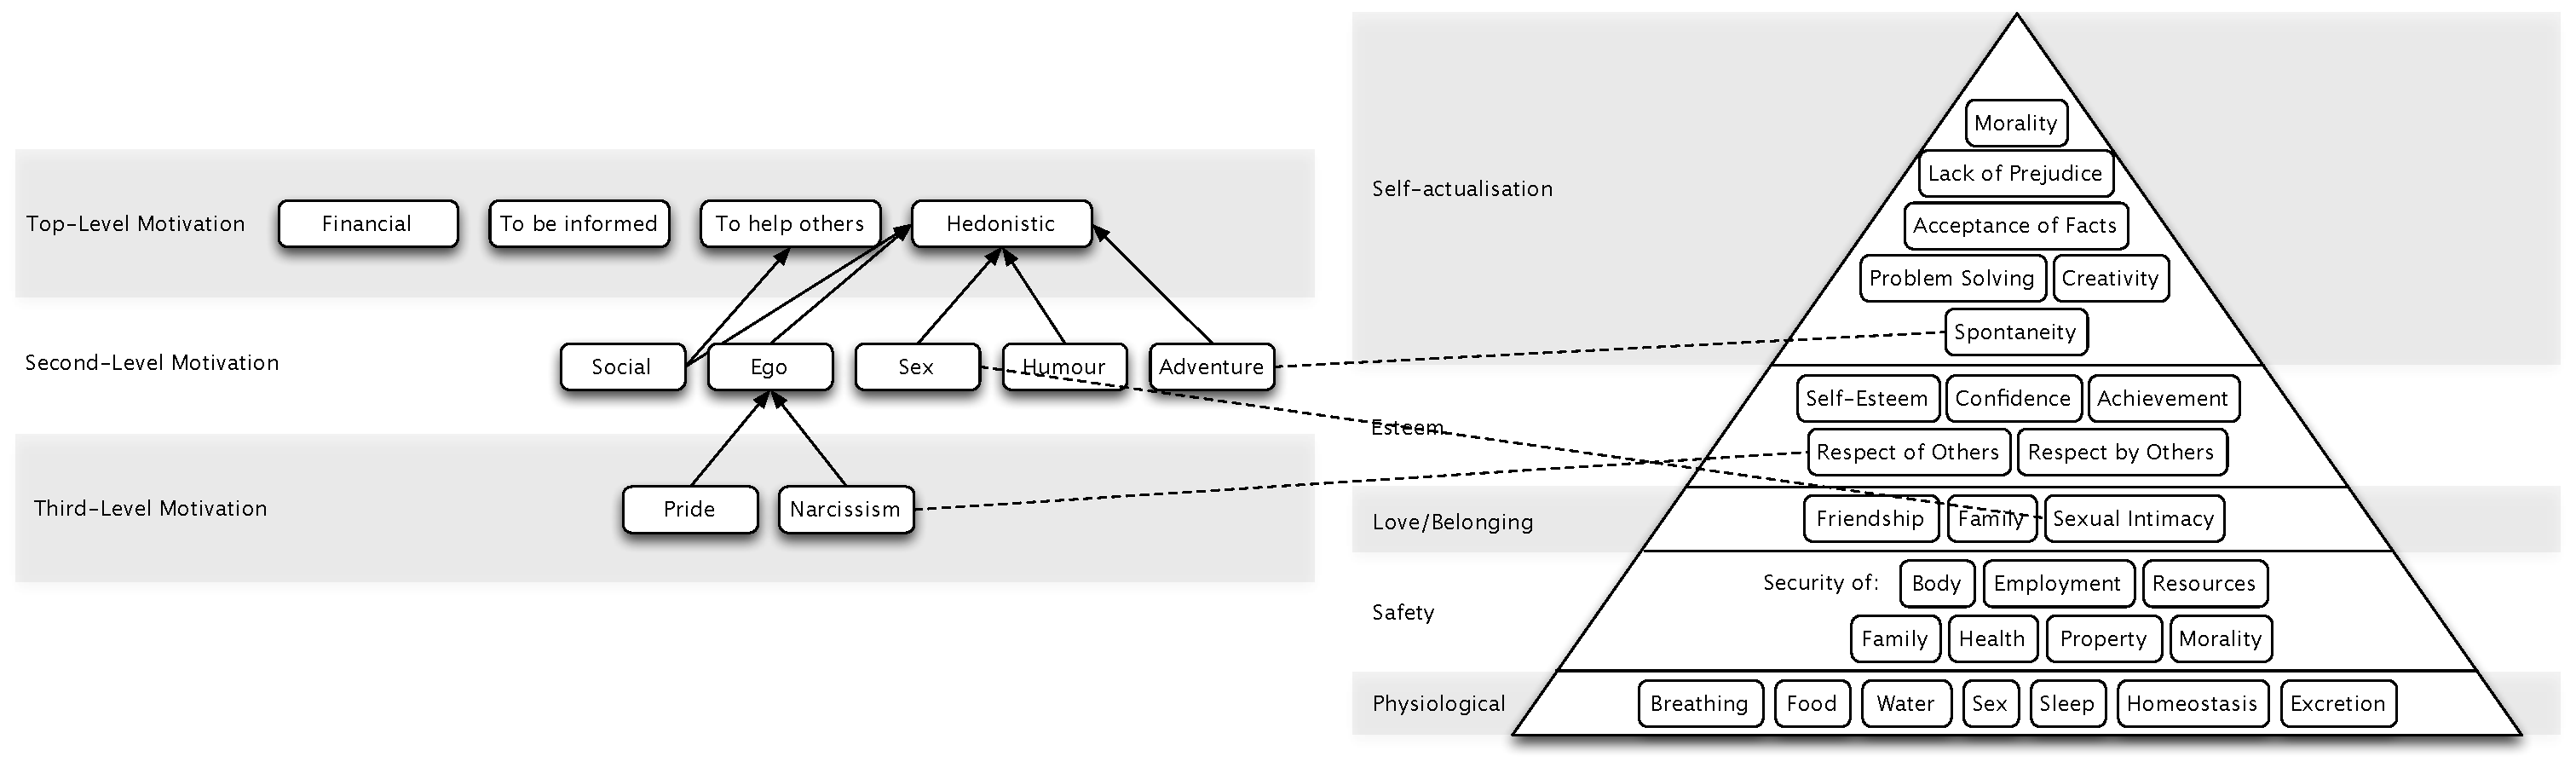
\includegraphics[width=18cm]{img/motivation.pdf}
%%\caption{Motivation hierarchy of participants using Social Machines, related to Maslow's hierarchy of needs.} \label{motivation}
%%\end{center}
%%\end{figure*}
%
%The motivations of users can be identified and mapped to existing human needs and motivations
%systems, such as Maslow's hierarchy of human needs~\cite{maslow} (e.g., self-actualisation, security
%respect of others). For each of these motivations, different roles that participate may have different {\it core motivations}, such as:
%
%\begin{enumerate}
%\item Benefit to contributor
%\item Benefit to moderator
%\item Benefit to system operator/host (e.g, Google, Facebook, Amazon)
%\item To affiliates of the host (e.g., Amazon affiliates, YouTube partners)
%\item To society as a whole
%\item To a contributor's social network
%\end{enumerate}
%
%In addition to relationships to Maslow's hierarchy of needs, which drive the motivations,
%we suggest that there are also resulting actions from each motivation. Thus, it should be
%possible to follow basic human needs to motivations in social machines, through to the
%actual actions (and therefore the necessary software feature support) that are made by
%participants in social machines. Our theory is that this path may enable designers of
%social machines to satisfy human needs by implemented specific features into their social
%machines, or to identify potential gaps in their serving of needs and motivations due
%to lack of implemented features.
%
%Motivation in specific social machines has been studied, including motivation of participants
%in: Wikipedia~\cite{kuznetsov2006motivations}; Open Source Software~\cite{lakhani2003hackers};
%Peer-to-peer filesharing~\cite{p2p}; Tagging~\cite{tagging}; and Virtual
%Communities~\cite{ardichvili2003motivation,Moore:2007:UMM:1235000.1235035}.
%
%[relate this work back to ours briefly.]


%\subsubsection{Artefacts of Social Machines}
%
%Our next observation was that there are a number of shared artefact types that can be classified within the context of social machines. Specifically that
%there are ``intentions'' that motivate the use of social machines, ``actions'' that are directly performed by participants of social machines, and ``contributions``
%that result from the use of social machines. We have taken these abstract concepts, and mapped them to a number of well-known social machines in order
%to demonstrate that these concepts can be used to compare and contrast different machines.
%
%[more here]


%\subsubsection{Metrics of participants and usage}
%
%Finally, we identified several constructs that are relevant for all social machines. First, there are construct that relate to ``analytics'' that can be measured at a point in time, and may change over time. We have documented these constructs in Table~\ref{table:constructs}. In the left column we list construct regarding the design affordances of the social machine. In the middle column we have a mixture of the result of how the design affordances actually were realised by the social computation, such as how users co-opted / incorporated / interpreted the constraints. Finally, in the right column we list analytical measures of social machines which are subject to change over time.

%% Constructs =============================================================


\subsection{Constructs}
The clustering process described in Section \ref{sec:methodology} yielded both a
reduction in the overall number of constructs (in particular an
elimination of over-represented areas) and the identification of three
simple themes: a

sets of constructs pertaining to users and roles within
each machine, second, the nature of tasks, problems and activities
performed through and using the machine, third, motivation for
participation, finally, the contexts of participation.

Each of these clusters contain between five and eight constructs as illustrated in Table
\ref{table:constructs}; we describe each of these themes in the
following subsections.

\begin{table}[htb]
\begin{center}
\begin{scriptsize}
\begin{tabular}{|p{8cm}|}
\hline
{\bf Tasks, purpose and context of participation} \\
\hline
Activities involve creative production of content \\
Activities involve subjective appraisal of content \\
Activities involve solving (a definable) computation task or set of problems\\
Tasks are domain-specific \\
The machine owner derives benefit from participation \\
Activities and tasks are pre-defined or participant-defined \\
Variation in types of contributions and tasks \\
Participants' participate to fulfil needs of a role \\
\hspace{1cm} work-related/professional role \\
\hspace{1cm} home/family related \\
\hspace{1cm} social role \\
\hspace{1cm} leisure/entertainment role \\
Participation is done via: \\
\hspace{1cm} mobile devices \\
\hspace{1cm} Web browsers \\
\hspace{1cm} apps \\
\hspace{1cm} sensors/sensing (location sensing and wearable devices) \\
Participation is done in a mobile context \\
\hspace{1cm} Physical location is relevant to the service \\
\hline
{\bf Participants and roles} \\
\hline
Generality of audience \\
Participant autonomy \\
Participant anonymity \\
Extent of hierarchical organisation of roles \\
Clear separation of roles among participants \\
\hline
{\bf Motivation and incentives} \\
\hline
Participants are intrinsically motivated:\\
\hspace{1cm} to gain/share knowledge \\
\hspace{1cm} to ``get something done'' \\
\hspace{1cm} to ``for fun/entertainment''\\
\hspace{1cm} to ``be social'' \\
\hspace{1cm} for the benefit of a specific group of people who need help \\
\hspace{1cm} for the benefit of society as a whole \\
Participation is motivated by extrinsic reward (payment, status) \\
\hline

\end{tabular}
\end{scriptsize}
\end{center}
\caption{Consolidated constructs of social machines} \label{table:constructs}
\end{table}

\subsubsection{Tasks, purpose, and context of participation}
The first set of constructs pertain to \emph{what} the participants
do, both individually within the system, and collectively as a whole.
Individual activities might include creation of content, subjective
appraisal of existing content, posing of problems, solving of
problems, and so on. The resulting `computation', looked at from a
macroscopic whole, might be the identification of high-quality
artistic content, insight, or creative works, collective problem
solving, and so on. Such tasks might be pre-defined by the system
designers, or brought to the system by participants. Further, these
tasks might be of a specific type or class, or of many varied types or
encompass a general class of activities. To capture this diversity,
we include a construct that differentiates machines with pre-defined problem spaces or are open to participant-provided tasks and activities. Finally, we ask whether the benefit derived by
participants is distinct from that gained by machine/platform owners
and service providers.

The second set of constructs pertains to the context(s) of each participant's greater (life-) activities in which the interaction with the system occurs. This context could be in a work context, home/family context, for leisure, and at a desk or away from a computer (in a mobile context). Participation could be conducted via apps, Web browsers, sensors and other technologies. Due to the predominance of geolocation services, one of the constructs collected through knowledge elicitation identifies the degree to which the user's location is used by the machine.

\subsubsection{Participants and roles}
This set of constructs pertain to the human participants of social machines and the way(s) participants are organised within them. One construct identifies whether participants constitute members of the general public, or are of a specific demographic, external group or organisation, occupation, or of a particular expertise. Two constructs, \emph{autonomy} and \emph{anonymity} pertain to the degree to which interaction is constrained among participants, and to the degree to which participants' identities are used and disclosed within the machine. Additional two constructs pertain to the roles: first, as to whether multiple roles are pre-differentiated by the machine or
whether all participants essentially initially assume the same role, second whether roles (pre-defined or emergent) are hierarchical.

\subsubsection{Motivation and incentives}
Related to the social structure motivation that sustains
continued participation in these systems. We identify six different
kinds of common sources of intrinsic motivation; first, that
participation is fun, second that it accomplishes an activity that the
participant enjoys or wanted to get done, third, that it satisfies the
desire to gain or share knowledge, or, fourth, or to be social. The
last two pertain to philanthropy, whether participation is seen to
benefit a particular group of disadvantaged people or individuals who
need assistance, or, finally, if participation is beneficial to
society as a whole. Finally, we ask whether extrinsic motivational
factors also contributed to sustained participation -- such factors
could include money reward, status, recognition and so on \cite{kuznetsov2006motivations,lakhani2003hackers,tagging}.
%Peer-to-peer filesharing~\cite{p2p}; Tagging~\cite{tagging}; and Virtual
%Communities~\cite{ardichvili2003motivation,Moore:2007:UMM:1235000.1235035}.

%% {\bf The types of tasks undertaken by the social component and the resulting contributions:}Social machines, just as any computing system, are built with a given purpose in mind, and exhibit functionality by which this purpose can be achieved. Users and the emerging social network interact with the system and with each other to carry out specific tasks by which they contribute to the `computation'. This includes the creation and refinement of digital artefacts by executing given actions, possibly in collaboration with other participants. For example, in GalaxyZoo\footnote{\url{http://www.galaxyzoo.org}} people classify galaxies with collective performance as good as professional astronomers, while in reCaptcha\footnote{\url{http://www.google.com/recaptcha}} they refine the data that describes digital manuscripts. Sometimes, systems look for innovative ways of getting people to engage with the systems, including game narratives, like in EteRNA\footnote{\url{http://eterna.cmu.edu}}, in which participants design RNA that is evaluated automatically using simulators and then refined via human effort, or monetary rewards, like in Amazon's Mechanical Turk, a platform in which users undertake routine (micro) tasks such as object classification, audio transcription and text translation.

% \subsubsection{Users and Roles}
% {\bf The roles of the participants and the social network they form}
% \subsubsection{Participation (How users interact with the Social Machine)}
%\subsubsection{Participation -- \emph{How and when user participate}}
%\subsubsection{Problems Solved and Benefit Derived}
%The result is what we call `participation' constructs. These constructs arise from use of a
%social machine, and are not necessarily predictable; they include:
%
%\begin{enumerate}
%\item {\bf Roles emerging in the social machine}
%  \newline In addition to designed and implemented roles such as {\it moderator} and {\it administrator}, emerging roles include motivations of the participant, such as {\it trolls}, {\it spammers}, {\it domain experts}, {\it social nexus}, and {\it re-blogger}.
%\item {\bf Quality of contributions}
%  \newline For any social machine, the quality of contributions will vary. While some
%    issues with quality can be predicted and protected against (e.g., through
%    multi-user result agreement on Mechanical Turk~\cite{ipeirotis2010quality}), some
%    particular issues with quality cannot always be predicted ahead of time.
%\item {\bf Content of contributions}
%    \newline While a system operator may design their social machine to generate specific
%    types of content, participants may subvert the system in order to generate other types,
%    or to concentrate on areas that were unforeseen at the time of launch, but are now seen
%    as useful to the operators. It is also possible that multiple social machines can be
%    combined/linked by users to further expand the types of contributions they produce.
%\item {\bf Global / cultural reach}
%    \newline A social machine may naturally focus on a narrow geographic area, for example
%    an Ushahidi-based social machine for local elections~\cite{meier2008crisis} or
%    natural disasters~\cite{morrow2011independent}. Such machines are unlikely to be
%    re-purposed by participants outside of that area. However, some machines have been
%    created for a single cultural/global area, but have potential global relevance that was
%    unforeseen early on. An example is the fall-off of English-language users of the
%    social network ``Orkut,'' which gained significant usage elsewhere, particularly in
%    Brazil.
%\item {\bf Task reach --- what do people use it for?}
%    \newline In addition to breaking cultural barriers, user have also shown that they can
%    use social machines for tasks that were not set up by the system operators. For example
%    the identification of ``Green Pea Galaxies'' using the GalaxyZoo social machine for
%    astronomy~\cite{greenpea}. Users were not originally asked to identify these types, but
%    a number of users identified them, and the software was modified to include them,
%    resulting in their discovery as a new type of galaxy.
%\item {\bf Active/Passive participation roles}
%    \newline When it comes to participation in social machines, there are levels of
%    participation that can be classified as being ``active'' and being ``passive.'' These
%    roles may not be particularly designed into systems, but may be exhibited over time.
%    Particularly noteworthy examples can be seen in news and link aggregation social
%    machines such as Reddit and Digg, where users can both submit links and vote on links.
%    The frequency of each of these activities can vary wildly, with a small
%    minority of users controlling the links that rise to the top~\cite{digg}.
%\end{enumerate}

\subsection{Using the classification framework}
\label{sec:usage}
In order to demonstrate usage of the constructs we ordered our social machines
by their Alexa ranking, and performed a full repertory grid elicitation exercise over the first $20$ of the $56$ collected in the first phase of the methodology (see Section \ref{sec:methodology}). This process assessing each social machine against the constructs by choosing a rate between $1$ and $5$. This led to a total of $680$ ratings, and the
results are illustrated in a grid and accompanying dendrograms for element and construct
similarity in Figure~\ref{dendrogram}.

\begin{figure}[htb]
\begin{center}
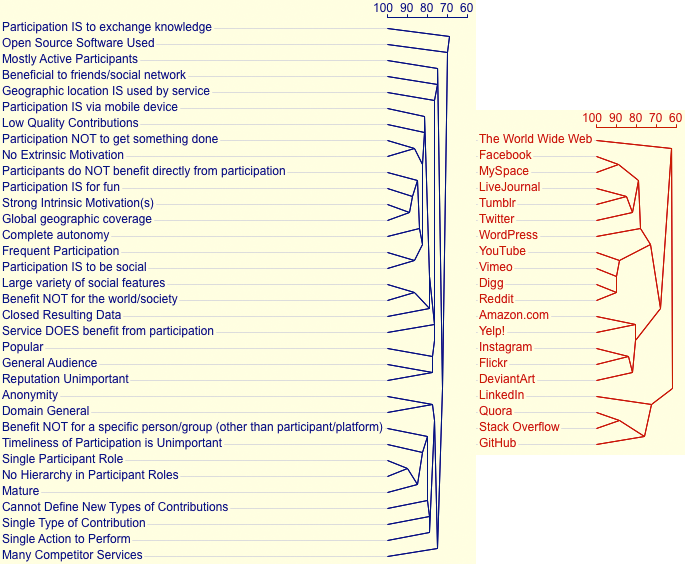
\includegraphics[width=0.5\textwidth]{img/dendrogram-both.png}
\caption{Dendrograms of constructs, in blue, and elements (social machines), in red, from a repertory grid exercise of the top $20$ (ranked by Alexa) social machines from our element set, against our consolidated constructs.} \label{dendrogram}
\end{center}
\end{figure}

%\begin{figure}[htb]
%\begin{center}
%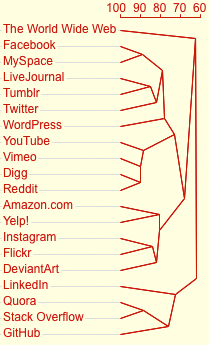
\includegraphics[width=0.2\textwidth]{img/dendrogram-elements.png}
%\caption{Dendrogram of elements (social machines) from a repertory grid exercise of the top $20$ (ranked by Alexa) social machines from our element set, against our consolidated constructs} \label{dendrogram}
%\end{center}
%\end{figure}
%
%\begin{figure}[htb]
%\begin{center}
%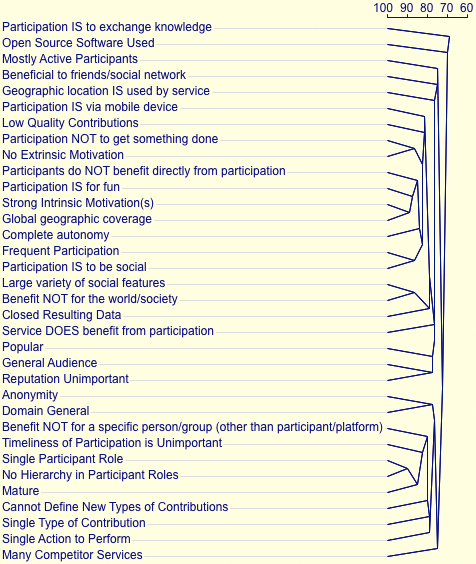
\includegraphics[width=0.4\textwidth]{img/dendrogram-constructs.png}
%\caption{Dendrogram of constructs from a repertory grid exercise of the top $20$ (ranked by Alexa) social machines from our element set, against our consolidated constructs} \label{dendrogram}
%\end{center}
%\end{figure}

From the dendrograms we can get a sense of similarities and separation of social machines. For
instance, it is clear that YouTube, Vimeo, Reddit, and Digg are similar, which is not unexpected, due to their focus on sharing content. Likewise, the exercise confirms commonalities between Quora and Stack Overflow, which can be easily understood, given their question answering purpose. There is also a dendrogram for the constructs, which can be used, as more data is collected, as an indicator for correlation between constructs. In this particular case, dendrogram suggests that there is a correlation between the `Single Participant Roles' and `No Hierarchy in Participant Roles' constructs, which is because they refer to the same aspect of social machines. Another, but less obvious connection is between the `Large variety of social features' and `Benefit NOT for the world/society', which requires further investigation.

We envisage three key use cases for our framework. First and foremost the framework forms the basis for a coherent and comprehensive description and classification of social machines. The knowledge elicitation technique referred to in this paper is just one of the many tools which can assist this exercise. In addition, it enables direct comparisons between systems, and provides a platform for terminologically consistent discussions about the field as a whole and specific instantiations. Finally, we also think that with more and more classification data becoming available, for instance, also through functionality that automatically monitors and computes the values of the some of the constructs introduced earlier, researchers will wish to apply prediction techniques (such as SVMs) to social machines, their behaviour, and impact.

\section{Future work: building a social machine around the classification framework}
In this paper we presented a first outline of a possible organisation structure for the design space of social machines. We introduced the key features of the notion of social machines, and explained how this notion differs from related areas such as collective intelligence, crowdsourcing and human computing. We then discussed the basic constructs of a classification framework created through the repertory grid elicitation technique. In its current version the framework consists of $31$ constructs clustered according to the main components of social machines: social and machine-driven services, and the interactions between them. Our future work will mostly be dedicated to the revision of this initial list of constructs. Most notably, we would like to add a number of constructs to emphasize the importance of the interaction aspect in the theory, engineering, and operation of social machines. This includes constructs related to the human-computer workflows supported (e.g., human intelligence replacing automatic algorithms as in GWAPs vs the different bots available on Wikipedia complementing collaborative manual editing), the way inputs from the crowd are validated, aggregated and turned into a useful outcome, as well as issues related collaboration and coordination, and interface and communication design. In addition, we plan to engage with the broader researcher community by setting up a social machine to facilitate discussions and feedback collection. One specific idea that is currently under development is to build a microtask-like environment, including specific game elements, in which participants are asked to provide answers to atomic challenges that rate and compare a pair of social machine instances according to a construct of our framework.



\section{Acknowledgments}
This work is supported under SOCIAM: The Theory and Practice of Social Machines. The SOCIAM Project is funded by the UK Engineering and Physical Sciences Research Council (EPSRC) under grant number EP/J017728/1 and comprises the Universities of Southampton, Oxford and Edinburgh.

%
% The following two commands are all you need in the
% initial runs of your .tex file to
% produce the bibliography for the citations in your paper.
\bibliographystyle{abbrv}
\bibliography{sigproc} % sigproc.bib is the name of the Bibliography in this case
% You must have a proper ".bib" file
% and remember to run:
% latex bibtex latex latex
% to resolve all references
%
% ACM needs `a single self-contained file'!
%
%APPENDICES are optional


\balancecolumns % GM June 2007
% That's all folks!
\end{document}
